\documentclass{beamer}

\usepackage[frenchb]{babel}
\usepackage[T1]{fontenc}
\usepackage[utf8]{inputenc}
\usepackage{listings}
\usepackage{color}
\usepackage{lmodern}
\usepackage{textcomp}

\definecolor{vertmoyen}{rgb}{0.25,0.45,0.10}
\definecolor{mygreen}{rgb}{0,0.6,0}
\definecolor{mygray}{rgb}{0.5,0.5,0.5}
\definecolor{mymauve}{rgb}{0.58,0,0.82}

\lstset{
    showstringspaces=false,
    breaklines=true,
    frameround=ffff,
    language=C,
    backgroundcolor=\color{white},
    commentstyle=\color{mygreen},
    keywordstyle=\color{blue},
    numberstyle=\tiny\color{mygray},
    rulecolor=\color{black},
    stringstyle=\color{mymauve},
    basicstyle=\ttfamily,
    stringstyle=\ttfamily,
    extendedchars=true,
    literate={é}{{\'e}}1 {è}{{\`e}}1 {à}{{\`a}}1 {ç}{{\c{c}}}1 {œ}{{\oe}}1 {ù}{{\`u}}1 {É}{{\'E}}1
    {È}{{\`E}}1 {À}{{\`A}}1 {Ç}{{\c{C}}}1 {Œ}{{\OE}}1 {Ê}{{\^E}}1 {ê}{{\^e}}1 {î}{{\^i}}1
    {ô}{{\^o}}1 {û}{{\^u}}1
}


\usetheme{Berlin}
% \setbeamerfont*{subsection in head/foot}{size=\huge}
\setbeamerfont*{section in head/foot}{size=\tiny}
\setbeamerfont*{subsection in head/foot}{size=\huge}
\setbeamerfont{headline}{size=\huge}
\setbeamercolor{structure}{fg=vertmoyen}
\setbeamertemplate{itemize item}[circle]



\title{
    Projet Système\\
    Compression Sans Perte
}
\author{Rémi GATTAZ - Julian HATTINGUAIS - Germain LECORPS - Reatha TITH}
\date{\today}

\begin{document}


\begin{frame}
\maketitle
\end{frame}

\begin{frame}
\tableofcontents
\end{frame}

\section{Cahier des Charges}

\begin{frame}
\begin{itemize}
\item Réversibilité
\item Marche pour tout fichier
\item Compresse selon les données du fichier
\item Prétraitement RLE
\item Possibilité de debug et traçage (trace très lourde pour les gros fichiers)
\item Temps de compression correct
\item Commandes faciles  utiliser
\end{itemize}
\end{frame}

\section{Organisation}

\begin{frame}
\begin{itemize}
\item Première journée de conception (aucune lignes de code)
\item Conception des différents modules (dico, binio, compression, décompression...)
\item Répartition du travail en binôme
\end{itemize}
\end{frame}


\section{LZW}

\subsection{Construction du dictionnaire}
\begin{frame}
 Besoins :
 \begin{enumerate}
  \item Compression : Arbre
  \item Décompression : Tableau
 \end{enumerate}
\end{frame}

\begin{frame}[containsverbatim]
\begin{columns}[t]
  \begin{column}{5cm}
  \begin{block}{Abre}
    \begin{lstlisting}
typedef struct _arbre {
  char valeur;
  Arbre* enfant;
  Arbre* frere;
  Arbre* parent;
  Code code;
} Arbre;
    \end{lstlisting}
  \end{block}
  \end{column}

  \begin{column}{5cm}
  \begin{block}{Dict}
    \begin{lstlisting}
typedef struct _dict {
  int nbElements;
  int tailleDico;
  Arbre** ids;
  Arbre* dico;
} Dict;
    \end{lstlisting}
  \end{block}
  \end{column}
 \end{columns}
\end{frame}


\subsection{Binio}
\begin{frame}[containsverbatim]
 binio -> traitement des fichiers\newline
 \newline
 Utilisation d'un buffer :
 \begin{block}{Buffer}
    \begin{lstlisting}
typedef struct s_buffer {
  char* content;
  char* courant;
  int significatif;
  int longeur;
} Buffer;
    \end{lstlisting}
  \end{block}


\end{frame}


\section{Prétraitement}

\subsection{Run Length Encoding}

\begin{frame}
Le codage se fait avec un automate à 2 états. On compare à chaque fois l'élément courant à l'élément précédent : si les deux sont égaux, on passe dans l'état 2 en incrémentant un compteur.
Le résultat du codage est de la forme suivante :\\
	$$abbbbcddddd -> 1a4b1c5d$$
Ainsi, pour un fichier où il y a peu de redondance, nous ajoutons un "1" devant chaque élément\\
Paquets max de 255
\end{frame}


\section{Commandes utiles}


\begin{frame}
- getopt\newline
- norme gnu\newline
Exemples :
    \begin{enumerate}
    \item ./LZW -c<file>
    \item ./LZW --compress=<file> -r
    \item ./LZW --rle -d<name>
    \item ./LZW --decompress=<file>
    \end{enumerate}
\end{frame}

\section{Tests}

\begin{frame}
    \begin{figure}[h]
    \centering
    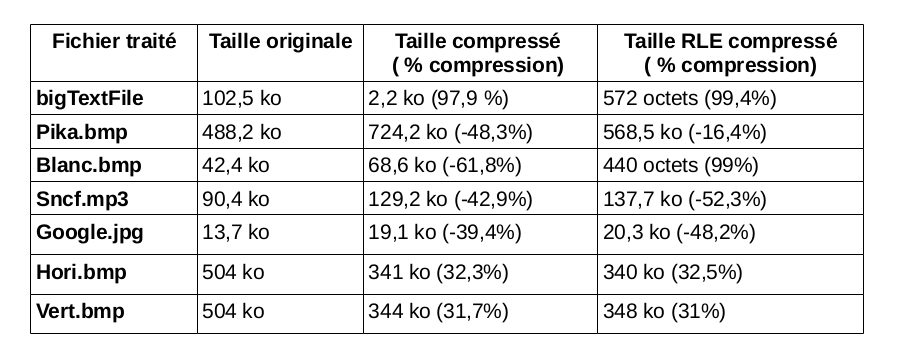
\includegraphics[scale=0.35]{tableau.png}
    \caption{Résultats pour différents fichiers et taux de compression}
    \label{resultats}
    \end{figure}
\end{frame}


\section{Problèmes rencontrés et évités}
\subsection{Difficultés}
\begin{frame}
 \begin{enumerate}
  \item Réinitialisation du dico
  \item Détection des erreurs de binio (test\_binio)
 \end{enumerate}
\end{frame}

\subsection{Facilités}
\begin{frame}
 \begin{enumerate}
  \item Répartition du travail (0 merge conflicts)
  \item Bonne conception
  \item Possiblité de changer de taille de dico très facilement
 \end{enumerate}
\end{frame}

\section{}
\begin{frame}
  \begin{center}
  \font\endfont = cmss10 at 12.40mm
  \color{Brown}
  \endfont
  \baselineskip 20.0mm
  Merci de votre attention
  \end{center}

\end{frame}

\end{document}
